\chapter{Ciclos de Vida}

\section{Ciclos estudados}
Um dos modelos é o Modelo Estrela de Hix e Hartson (\citeyear{hix}). Esse ciclo de vida que possui como fases: Avaliação, Requisitos, Análise de tarefas, 
Implementação, Protótipo e Projeto Conceitual. Esse modelo é centrado na avaliação do usuário, sendo essa uma fase que se repete no ciclo de vida após cada uma das fases.
Isso acontece, pois é necessário que o usuário avalie cada etapa do processo para que o produto final atenda de forma efetiva às suas necessidades.

O outro modelo, apresentado por Preece, Rogers e Sharp (\citeyear{preece}), consiste no ciclo de vida da engenharia de usabilidade, suas fases estão bem acopladas às fases 
do desenvolvimento de software. Trata-se de um modelo que é composto de três fases: análise dos requisitos, projeto/teste/desenvolvimento e instalação, todavia 
cada atividade dessa é dividida em muitas tarefas detalhadas. Essas fases possuem algumas atividades como: Conheça seu usuário, realize uma análise competitiva, 
defina as metas de usabilidade, faça designs paralelos, adote o design participativo, faça o design coordenado da interface como um todo, aplique diretrizes, 
faça protótipos e realize testes empíricos. A partir disso, é possível perceber que este modelo também pode ser considerado focado no usuário, e que possui uma 
característica iterativa.

Barbosa e Silva (\citeyear{BARBOSA}) trazem outros quatro processos de design: Design Contextual, Design Baseado em Cenários, Design Dirigido por Objetivos e Design Centrado na 
Comunicação. O Design Contextual tem como forte característica a análise do contexto no qual o usuário está inserido. Tem como atividades básicas a investigação contextual,
a modelagem do trabalho, a consolidação da modelagem do trabalho, reprojetar o trabalho, o projeto do ambiente do usuário, a prototipação e os testes com os usuários.

O Design baseado em cenários “é um processo que utiliza diferentes tipos de cenários como representação básica e fundamental durante todas as atividades envolvidas 
na concepção de uma solução de IHC.” (ROSSON E CAROL, 2002 apud \cite{BARBOSA}). Dessa forma, a análise de cada cenário permite ao projetista avaliar como o 
sistema será utilizado, e quais são as necessidades que o sistema deve atender em determinada situação. Nesse modelo, as atividades são: analisar, projetar e prototipar 
e avaliar.

No Design Dirigido por Objetivos o foco são as tecnologias existentes como auxílio para alcançar o objetivo final. Esse processo tem foco tanto no usuário como na
experiência do design no uso do modelo. Consiste em seis fases: pesquisar, modelar, definir requisitos, projetar, refinar e manter. \cite{BARBOSA}

Por último, o Design Centrado na Comunicação que consiste na preocupação da melhor comunicação entre interface e usuário. Assim, esse modelo preza pela busca de uma
alta interatividade. Possui três fases: análise, projeto de interação e interface e avaliação. \cite{BARBOSA}

\section{Ciclo escolhido}
Para este projeto o modelo adotado será o Modelo Estrela, que pode ser visto na Figura \ref{ciclo}, pois está concentrado na avaliação do usuário. Isso acontece, pois é necessário que o usuário avalie cada 
etapa do processo para que o produto final atenda de forma efetiva suas necessidades, e esse é o objetivo do MyPush, atender de forma efetiva as necessidades de seus
usuários. Embora outros modelos também estejam concentrados na avaliação, esse modelo é relativamente mais simples e também permite uma maior flexibilidade em relação a
ordem das etapas. 

\begin{figure}[!h]
 \centering
 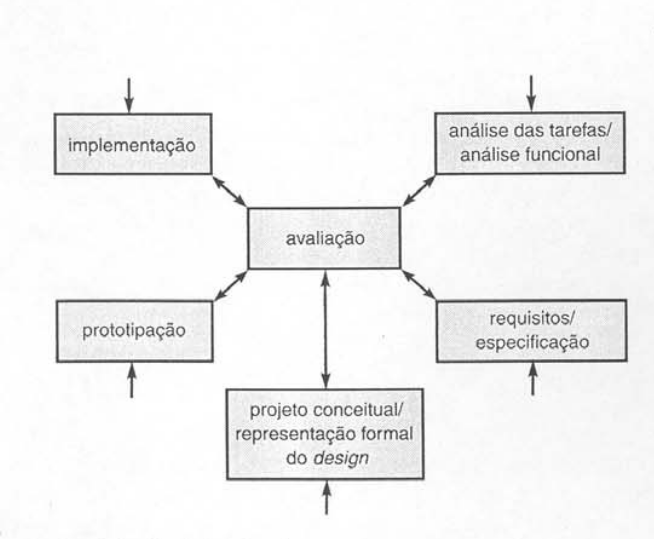
\includegraphics[scale=0.5]{figuras/modelo_estrela.png}
 \caption{Modelo de ciclo de vida estrela. Fonte: \cite{preece}}
 \label{ciclo}
\end{figure}